% questions.tex —— 2021 年·全国甲卷·文科 · 题目内容片段（无答案）
% 由 tools/generate_projects.py 依来源总账自 2021/2021_数学真题_全国甲文_试题.md 生成，勿手改（改源 MD 后重跑）


\begin{gknotice}
\textbf{卷别说明}：上游 PDF 页眉逐字印「2021 普通高等学校招生考试 (全国卷 II 文)」，与文件名及适用省份标注的「全国甲卷」不一致。经核查，2021 年全国甲卷适用云南、四川、广西、贵州、西藏，其前身为全国Ⅲ卷而非Ⅱ卷，故页眉卷别标签为上游沿用旧模板所致。本文按文件名与省份列表定卷别，页眉原文照录不改。详见问题总账中的身份条目。

\textbf{结构提示}：本卷为文理分科时期的 23 题制，第 22、23 题为选考题（极坐标与参数方程／不等式选讲），\textbf{二选一作答}。
\end{gknotice}

\par\medskip

\gkpart{一、选择题}

\begin{gktip}
本题共 12 小题，每小题 5 分，共 60 分。在每小题给出的四个选项中，只有一项是符合题目要求的。
\end{gktip}

\begin{question}
\gkti{1}设集合 $M=\{1,3,5,7,9\}$，$N=\{x\mid 2x>7\}$，则 $M\cap N=$\mbox{（　　）}

\begin{gkopts}(4)
\task A．$\{7,9\}$
\task B．$\{5,7,9\}$
\task C．$\{3,5,7,9\}$
\task D．$\{1,3,5,7,9\}$
\end{gkopts}

\Needspace{0.4\textheight}
\end{question}
\begin{question}
\gkti{2}为了解某地农村经济情况，对该地农户家庭年收入进行抽样调查，将农户家庭年收入的调查数据整理得到如下频率分布直方图：
\nopagebreak[4]
\begin{center}% 2021 全国甲卷文科 2：农户家庭年收入的频率分布直方图
% 绘制依据：源 PDF 第 1 页原图。纵轴「频率/组距」，横轴「收入/万元」。
% 横轴刻度 0 与 2.5,3.5,…,14.5；纵轴标注 0.02、0.04、0.10、0.14、0.20。
% 十二个组距均为 1，自 2.5 起各组高度依次为
%   0.02, 0.04, 0.10, 0.14, 0.20, 0.20, 0.10, 0.10, 0.04, 0.02, 0.02, 0.02。
% 交叉验算（四项独立约束全部吻合，故读数可靠）：
%   Σ高度×1 = 1.00；低于 4.5 者 0.02+0.04 = 6%（选项 A）；
%   不低于 10.5 者 0.04+0.02×3 = 10%（选项 B）；4.5~8.5 者 0.64 > 0.5（选项 D）；
%   均值 Σ组中值×频率 = 7.68 > 6.5（选项 C 故为「不正确」者）。
% 版式：横轴 0 与首刻度 2.5 之间画断轴锯齿；每个纵轴标注值处引水平虚线至对应柱顶。
\begin{tikzpicture}[font=\small]
  % x: 1 单位收入 = 0.62cm，自 2.5 起；y: 0.02 = 0.42cm
  \def\xs{0.62}\def\ys{21.0}
  \pgfmathsetmacro{\xz}{0.55}% 断轴后横轴起点（对应收入 2.5）
  % 断轴的横轴
  \draw (0,0) -- (0.10,0);
  \draw (0.10,0) -- (0.16,0.10) -- (0.26,-0.10) -- (0.32,0);
  \draw[->] (0.32,0) -- ({\xz+12*\xs+0.75},0);
  \node[anchor=north] at (0,-0.06) {$0$};
  \node[anchor=west] at ({\xz+12*\xs+0.30},0.26) {收入$/$万元};
  % 纵轴
  \draw[->] (0,0) -- (0,{0.20*\ys+0.85});
  \node[anchor=south east, align=right] at (0.06,{0.20*\ys+0.30}) {频率\\[-2pt]\rule{1.1cm}{0.4pt}\\[-2pt]组距};
  % 纵轴标注与引至柱顶的水平虚线
  \foreach \v/\xend in {0.02/12, 0.04/9, 0.10/7, 0.14/4, 0.20/3} {
    \node[anchor=east, inner sep=2pt] at (-0.04,{\v*\ys}) {$\v$};
    \draw[dashed, gray] (0,{\v*\ys}) -- ({\xz+\xend*\xs},{\v*\ys});
  }
  % 十二个矩形
  \foreach \i/\h in {0/0.02, 1/0.04, 2/0.10, 3/0.14, 4/0.20, 5/0.20,
                     6/0.10, 7/0.10, 8/0.04, 9/0.02, 10/0.02, 11/0.02} {
    \draw ({\xz+\i*\xs},0) rectangle ({\xz+(\i+1)*\xs},{\h*\ys});
  }
  % 横轴刻度标注
  \foreach \i/\t in {0/2.5, 1/3.5, 2/4.5, 3/5.5, 4/6.5, 5/7.5, 6/8.5,
                     7/9.5, 8/10.5, 9/11.5, 10/12.5, 11/13.5, 12/14.5} {
    \node[anchor=north, inner sep=2pt, font=\tiny] at ({\xz+\i*\xs},-0.06) {$\t$};
  }
\end{tikzpicture}
\end{center}
\nopagebreak[4]
根据此频率分布直方图，下面结论中不正确的是\mbox{（　　）}

\begin{gkopts}(1)
\task A．该地农户家庭年收入低于 $4.5$ 万元的农户比率估计为 $6\%$
\task B．该地农户家庭年收入不低于 $10.5$ 万元的农户比率估计为 $10\%$
\task C．估计该地农户家庭年收入的平均值不超过 $6.5$ 万元
\task D．估计该地有一半以上的农户，其家庭年收入介于 $4.5$ 万元至 $8.5$ 万元之间
\end{gkopts}

\end{question}
\begin{question}
\gkti{3}已知 $(1-\mathrm i)^{2}z=3+2\mathrm i$，则 $z=$\mbox{（　　）}

\begin{gkopts}(2)
\task A．$-1-\dfrac32\mathrm i$
\task B．$-1+\dfrac32\mathrm i$
\task C．$-\dfrac32+\mathrm i$
\task D．$-\dfrac32-\mathrm i$
\end{gkopts}

\end{question}
\begin{question}
\gkti{4}下列函数中是增函数的为\mbox{（　　）}

\begin{gkopts}(2)
\task A．$f(x)=-x$
\task B．$f(x)=\left(\dfrac23\right)^{x}$
\task C．$f(x)=x^{2}$
\task D．$f(x)=\sqrt[3]{x}$
\end{gkopts}

\end{question}
\begin{question}
\gkti{5}点 $(3,0)$ 到双曲线 $\dfrac{x^{2}}{16}-\dfrac{y^{2}}9=1$ 的一条渐近线的距离为\mbox{（　　）}

\begin{gkopts}(4)
\task A．$\dfrac95$
\task B．$\dfrac85$
\task C．$\dfrac65$
\task D．$\dfrac45$
\end{gkopts}

\end{question}
\begin{question}
\gkti{6}青少年视力是社会普遍关注的问题，视力情况可借助视力表测量。通常用五分记录法和小数记录法记录视力数据，五分记录法的数据 $L$ 和小数记录法的数据 $V$ 满足 $L=5+\lg V$。已知某同学视力的五分记录分的数据为 $4.9$，则其视力的小数记录法的数据约为（$\sqrt[10]{10}\approx1.259$）\mbox{（　　）}

\begin{gkopts}(4)
\task A．$1.5$
\task B．$1.2$
\task C．$0.8$
\task D．$0.6$
\end{gkopts}

\Needspace{0.4\textheight}
\end{question}
\begin{question}
\gkti{7}在一个正方体中，过顶点 $A$ 的三条棱的中点分别为 $E$，$F$，$G$。该正方体截去三棱锥 $A\text{-}EFG$ 后，所得多面体的三视图中，正视图如图所示，则相应的侧视图是\mbox{（　　）}
\nopagebreak[4]
\begin{center}% 2021 全国甲卷文科 7：正视图与四个候选侧视图
% 绘制依据：源 PDF 第 1 页原图，400 dpi 放大逐个量取。五个同样大小的正方形。
% 关键几何：所有截线都是【边中点到边中点】——与题设 E、F、G 为过顶点 A 的三条棱
% 的中点相吻合，故截面在各投影面上的像必落在相邻两边的中点连线上。
%   正视图：【虚线】自左边中点降至底边中点，切掉【左下角】。
%   (A) 实线，自底边中点升至右边中点，切【右下角】
%   (B) 虚线，自左边中点降至底边中点，切【左下角】——与正视图同形，是「照抄正视图」的陷阱项
%   (C) 虚线，自底边中点升至右边中点，切【右下角】
%   (D) 实线，自左边中点降至底边中点，切【左下角】
% ⚠️ 初版曾把正视图与 (B)(D) 的下端画到约 0.88 宽处而非底边中点，属实质失真
%    （会改变「切哪个角」的判读）；已按 400 dpi 原图量取修正为严格中点。
% 选项标签 (A)~(D) 置于各正方形左下角外侧。
\begin{tikzpicture}[font=\small, line width=0.4pt]
  \def\s{1.75}% 正方形边长
  % 两种截线：切左下角（左边中点→底边中点）、切右下角（底边中点→右边中点）
  % #1 线型选项
  \newcommand{\cutLL}[1][]{\draw[#1] (0,{0.5*\s}) -- ({0.5*\s},0);}
  \newcommand{\cutLR}[1][]{\draw[#1] ({0.5*\s},0) -- (\s,{0.5*\s});}
  % ---------- 正视图 ----------
  \begin{scope}[shift={({1.6*\s},{1.75*\s})}]
    \draw (0,0) rectangle (\s,\s);
    \cutLL[dashed]
    \node[anchor=north] at ({0.5*\s},-0.10) {正视图};
  \end{scope}
  % ---------- 四个选项 ----------
  \begin{scope}[shift={(0,0)}]
    \draw (0,0) rectangle (\s,\s);  \cutLR
    \node[anchor=east] at (-0.06,{0.06*\s}) {(A)};
  \end{scope}
  \begin{scope}[shift={({1.55*\s},0)}]
    \draw (0,0) rectangle (\s,\s);  \cutLL[dashed]
    \node[anchor=east] at (-0.06,{0.06*\s}) {(B)};
  \end{scope}
  \begin{scope}[shift={({3.10*\s},0)}]
    \draw (0,0) rectangle (\s,\s);  \cutLR[dashed]
    \node[anchor=east] at (-0.06,{0.06*\s}) {(C)};
  \end{scope}
  \begin{scope}[shift={({4.65*\s},0)}]
    \draw (0,0) rectangle (\s,\s);  \cutLL
    \node[anchor=east] at (-0.06,{0.06*\s}) {(D)};
  \end{scope}
\end{tikzpicture}
\end{center}
\nopagebreak[4]
\end{question}
\begin{question}
\gkti{8}在 $\triangle ABC$ 中，已知 $B=120^\circ$，$AC=\sqrt{19}$，$AB=2$，则 $BC=$\mbox{（　　）}

\begin{gkopts}(4)
\task A．$1$
\task B．$\sqrt2$
\task C．$\sqrt5$
\task D．$3$
\end{gkopts}

\end{question}
\begin{question}
\gkti{9}记 $S_n$ 为等比数列 $\{a_n\}$ 的前 $n$ 项和。若 $S_2=4$，$S_4=6$，则 $S_6=$\mbox{（　　）}

\begin{gkopts}(4)
\task A．$7$
\task B．$8$
\task C．$9$
\task D．$10$
\end{gkopts}

\end{question}
\begin{question}
\gkti{10}将 $3$ 个 $1$ 和 $2$ 个 $0$ 随机排成一行，则 $2$ 个 $0$ 不相邻的概率为\mbox{（　　）}

\begin{gkopts}(4)
\task A．$0.3$
\task B．$0.5$
\task C．$0.6$
\task D．$0.8$
\end{gkopts}

\end{question}
\begin{question}
\gkti{11}若 $\alpha\in\left(0,\dfrac\pi2\right)$，$\tan2\alpha=\dfrac{\cos\alpha}{2-\sin\alpha}$，则 $\tan\alpha=$\mbox{（　　）}

\begin{gkopts}(2)
\task A．$\dfrac{\sqrt{15}}{15}$
\task B．$\dfrac{\sqrt5}5$
\task C．$\dfrac{\sqrt5}3$
\task D．$\dfrac{\sqrt{15}}5$
\end{gkopts}

\end{question}
\begin{question}
\gkti{12}设 $f(x)$ 是定义域为 $\mathbf R$ 的奇函数，且 $f(1+x)=f(-x)$。若 $f\left(-\dfrac13\right)=\dfrac13$，则 $f\left(\dfrac53\right)=$\mbox{（　　）}

\begin{gkopts}(4)
\task A．$-\dfrac53$
\task B．$-\dfrac13$
\task C．$\dfrac13$
\task D．$\dfrac53$
\end{gkopts}

\par\medskip

\end{question}
\gkpart{二、填空题}

\begin{gktip}
本题共 4 小题，每小题 5 分，共 20 分。
\end{gktip}

\begin{question}
\gkti{13}若向量 $\boldsymbol a$，$\boldsymbol b$ 满足 $|\boldsymbol a|=3$，$|\boldsymbol a-\boldsymbol b|=5$，$\boldsymbol a\cdot\boldsymbol b=1$，则 $|\boldsymbol b|=$ \gkblank{}．

\end{question}
\begin{question}
\gkti{14}已知一个圆锥的底面半径为 $6$，其体积为 $30\pi$，则该圆锥的侧面积为 \gkblank{}．

\Needspace{0.4\textheight}
\end{question}
\begin{question}
\gkti{15}已知函数 $f(x)=2\cos(\omega x+\varphi)$ 的部分图象如图所示，则 $f\left(\dfrac\pi2\right)=$ \gkblank{}．
\nopagebreak[4]
\begin{center}% 2021 全国甲卷文科 15：f(x)=2cos(ωx+φ) 的部分图象
% 绘制依据：源 PDF 第 1 页原图。由图上两处标注反解出解析式：
%   π/3 处为【下降零点】，13π/12 处为【最大值】（虚线引至 y=2）。
%   下降零点到次个最大值恰为 3T/4，故 3T/4 = 13π/12 − π/3 = 3π/4，得 T = π、ω = 2；
%   再由 13π/12 为最大值定 φ = −π/6，即 f(x) = 2cos(2x − π/6)。
%   回验：首个最大值在 x = π/12（恰在 O 右侧，与图一致）；
%         x = π/3 处相位为 π/2（值为零且下降，与图一致）。
% 关键点位：最大值 π/12≈0.262 与 13π/12≈3.403；下降零点 π/3≈1.047；
%           最小值 7π/12≈1.833；上升零点 5π/6≈2.618。
% 标注：y 轴「2」；x 轴 O、π/3、13π/12；y=2 处水平虚线引至右侧峰；
%       13π/12 处竖直虚线自 x 轴引至峰顶。无刻度线、无网格。
\begin{tikzpicture}
\begin{axis}[width=10.4cm, height=5.6cm, font=\small,
  axis lines=middle, xlabel={$x$}, ylabel={$y$},
  xmin=-0.75, xmax=4.75, ymin=-2.85, ymax=2.95,
  xtick=\empty, ytick=\empty, clip=false,
  every axis x label/.style={at={(current axis.right of origin)}, anchor=west},
  every axis y label/.style={at={(current axis.above origin)}, anchor=south}]
  % y=2 水平虚线（自 y 轴引至右侧峰）与 13π/12 竖直虚线
  \addplot[dashed, domain=0:3.40339, samples=2] {2};
  \draw[dashed] (axis cs:3.40339,0) -- (axis cs:3.40339,2);
  % 曲线本体
  \addplot[domain=-0.42:4.42, samples=300, thick] {2*cos(deg(2*x-pi/6))};
  % 标注
  \node[anchor=east, inner sep=2pt] at (axis cs:-0.05,2) {$2$};
  \node[anchor=north east, inner sep=2pt] at (axis cs:-0.03,-0.04) {$O$};
  \node[anchor=north, inner sep=3pt] at (axis cs:1.04720,-0.05) {$\frac{\pi}{3}$};
  \node[anchor=north, inner sep=3pt] at (axis cs:3.40339,-0.05) {$\frac{13\pi}{12}$};
\end{axis}
\end{tikzpicture}
\end{center}
\nopagebreak[4]
\end{question}
\begin{question}
\gkti{16}已知 $F_1$，$F_2$ 为椭圆 $C:\dfrac{x^{2}}{16}+\dfrac{y^{2}}4=1$ 的两个焦点，$P$，$Q$ 为 $C$ 上关于坐标原点对称的两点，且 $|PQ|=|F_1F_2|$，则四边形 $PF_1QF_2$ 的面积为 \gkblank{}．

\par\medskip

\end{question}
\gkpart{三、解答题}

\begin{gktip}
共 70 分。解答应写出文字说明、证明过程或演算步骤。第 17～21 题为必考题，每个试题考生都必须作答。第 22、23 题为选考题，考生根据要求作答。
\end{gktip}

\gksubpart{（一）必考题：共 60 分。}

\begin{question}
\gkti{17}\textbf{（12 分）} 甲、乙两台机床生产同种产品，产品质量分为一级品和二级品，为了比较两台机床产品的质量，分别用两台机床各生产了 $200$ 件产品，产品的质量情况统计如下表：

\begin{center}
\begin{tabular}{cccc}
\toprule
 & 一级品 & 二级品 & 合计 \\
\midrule
甲机床 & $150$ & $50$ & $200$ \\
乙机床 & $120$ & $80$ & $200$ \\
合计 & $270$ & $130$ & $400$ \\
\bottomrule
\end{tabular}
\end{center}

  (1) 甲机床、乙机床生产的产品中一级品的频率分别是多少？

  (2) 能否有 $99\%$ 的把握认为甲机床的产品质量与乙机床的产品质量有差异？

\Needspace{10\baselineskip}
  附：$K^{2}=\dfrac{n(ad-bc)^{2}}{(a+b)(c+d)(a+c)(b+d)}$，

\begin{center}
\begin{tabular}{cccc}
\toprule
$P(K^{2}\geqslant k)$ & $0.050$ & $0.010$ & $0.001$ \\
\midrule
$k$ & $3.841$ & $6.635$ & $10.828$ \\
\bottomrule
\end{tabular}
\end{center}

\end{question}
\begin{question}
\gkti{18}\textbf{（12 分）} 记 $S_n$ 为数列 $\{a_n\}$ 的前 $n$ 项和。已知 $a_n>0$，$a_2=3a_1$，且数列 $\left\{\sqrt{S_n}\right\}$ 是等差数列，证明：$\{a_n\}$ 是等差数列。

\Needspace{0.4\textheight}
\end{question}
\begin{question}
\gkti{19}\textbf{（12 分）} 已知直三棱柱 $ABC\text{-}A_1B_1C_1$ 中，侧面 $AA_1B_1B$ 为正方形，$AB=BC=2$，$E$，$F$ 分别为 $AC$ 和 $CC_1$ 的中点，$BF\perp A_1B_1$。
\nopagebreak[4]
\begin{center}% 2021 全国甲卷文科 19：直三棱柱 ABC-A₁B₁C₁，E 为 AC 中点、F 为 CC₁ 中点、D 在棱 A₁B₁ 上
% 绘制依据：源 PDF 第 2 页原图。斜投影：AB 为后棱（水平），C 为前顶点（画在下方偏中）。
% 顶点坐标（图纸坐标，非题设长度）：
%   A₁(0,3.00) B₁(2.60,3.00) C₁(1.35,2.35)；A(0,0.55) B(2.60,0.55) C(1.35,-0.10)
%   D 在 A₁B₁ 上偏 B₁ 一侧：(2.15,3.00)
%   E = (A+C)/2 = (0.675,0.225)；F = (C+C₁)/2 = (1.35,1.125)
%   （E、F 由中点关系算出，与原图标注位置吻合，故坐标系可信。）
% 线型：可见棱实线；被遮挡的后底棱 AB 与内部辅助线 EB、DE 用虚线。
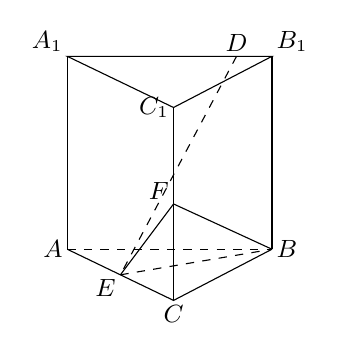
\begin{tikzpicture}[font=\small, line width=0.4pt,
  every node/.style={inner sep=1.5pt}]
  \coordinate (A1) at (0,3.00);   \coordinate (B1) at (2.60,3.00);
  \coordinate (C1) at (1.35,2.35);
  \coordinate (A)  at (0,0.55);   \coordinate (B)  at (2.60,0.55);
  \coordinate (C)  at (1.35,-0.10);
  \coordinate (D)  at (2.15,3.00);
  \coordinate (E)  at (0.675,0.225);
  \coordinate (F)  at (1.35,1.125);
  % 上底面
  \draw (A1) -- (B1) -- (C1) -- cycle;
  % 侧棱
  \draw (A1) -- (A);  \draw (B1) -- (B);  \draw (C1) -- (C);
  % 下底面：后棱 AB 被遮挡
  \draw[dashed] (A) -- (B);
  \draw (A) -- (C) -- (B);
  % 辅助线
  \draw (B) -- (F);          % BF
  \draw (E) -- (F);          % EF（三棱锥 F-EBC 的棱）
  \draw[dashed] (E) -- (B);  % EB（内部，被遮挡）
  \draw[dashed] (D) -- (E);  % DE
  % 顶点标注
  \node[anchor=south east] at (A1) {$A_1$};
  \node[anchor=south west] at (B1) {$B_1$};
  \node[anchor=south]      at (D)  {$D$};
  \node[anchor=east]       at (C1) {$C_1$};
  \node[anchor=east]       at (A)  {$A$};
  \node[anchor=west]       at (B)  {$B$};
  \node[anchor=north]      at (C)  {$C$};
  \node[anchor=north east] at (E)  {$E$};
  \node[anchor=south east] at (F)  {$F$};
\end{tikzpicture}
\end{center}
\nopagebreak[4]
  (1) 求三棱锥 $F\text{-}EBC$ 的体积；

  (2) 已知 $D$ 为棱 $A_1B_1$ 上的点，证明：$BF\perp DE$。

\end{question}
\begin{question}
\gkti{20}\textbf{（12 分）} 设函数 $f(x)=a^{2}x^{2}+ax-3\ln x+1$，其中 $a>0$。

  (1) 讨论 $f(x)$ 的单调性；

  (2) 若 $y=f(x)$ 的图象与 $x$ 轴没有公共点，求 $a$ 的取值范围。

\end{question}
\begin{question}
\gkti{21}\textbf{（12 分）} 抛物线 $C$ 的顶点为坐标原点 $O$，焦点在 $x$ 轴上，直线 $l:x=1$ 交 $C$ 于 $P$，$Q$ 两点，且 $OP\perp OQ$。已知点 $M(2,0)$，且 $\odot M$ 与 $l$ 相切。

  (1) 求 $C$，$\odot M$ 的方程；

  (2) 设 $A_1$，$A_2$，$A_3$ 是 $C$ 上的三个点，直线 $A_1A_2$，$A_1A_3$ 均与 $\odot M$ 相切。判断 $A_2A_3$ 与 $\odot M$ 的位置关系，并说明理由。

\end{question}
\gksubpart{（二）选考题：共 10 分。请考生在第 22、23 两题中任选一题作答。如果多做，则按所做的第一题计分。}

\begin{question}
\gkti{22}\textbf{（10 分）选修 4—4：坐标系与参数方程} 

在直角坐标系 $xOy$ 中，以坐标原点为极点，$x$ 轴正半轴为极轴建立极坐标系，曲线 $C$ 的极坐标方程为 $\rho=2\sqrt2\cos\theta$。

  (1) 将 $C$ 的极坐标方程化为直角坐标方程；

  (2) 设点 $A$ 的直角坐标为 $(1,0)$，$M$ 为 $C$ 上的动点，点 $P$ 满足 $\overrightarrow{AP}=\sqrt2\,\overrightarrow{AM}$，写出 $P$ 的轨迹 $C_1$ 的参数方程，并判断 $C$ 与 $C_1$ 是否有公共点。

\Needspace{0.4\textheight}
\end{question}
\begin{question}
\gkti{23}\textbf{（10 分）选修 4—5：不等式选讲} 

已知函数 $f(x)=|x-2|$，$g(x)=|2x+3|-|2x-1|$。
\nopagebreak[4]
\begin{center}% 2021 全国甲卷文科 23：供考生作图用的空白方格坐标系
% 绘制依据：源 PDF 第 2 页原图。整幅为方格网，坐标轴过原点，
% 网格以原点为中心，左右、上下各 8 格，仅标注 O 与两轴上的 1。
% 本图无曲线内容——它是题目要求「画出 y=f(x) 和 y=g(x) 的图象」的作图区。
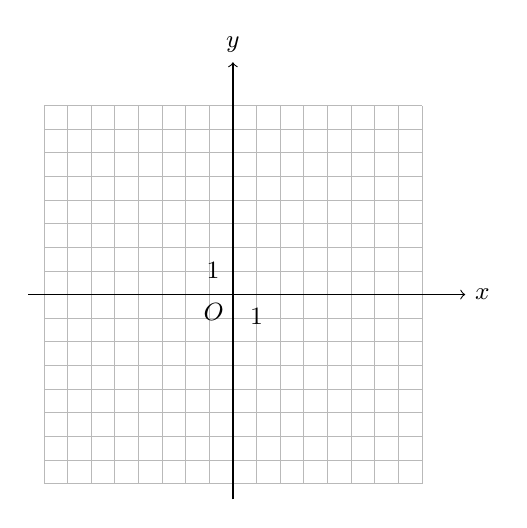
\begin{tikzpicture}[font=\small, line width=0.4pt]
  \def\u{0.30}% 单位格边长；紧凑印刷版保留 16×16 作图区并适度缩小
  \pgfmathsetmacro{\xa}{-8}\pgfmathsetmacro{\xb}{8}
  \pgfmathsetmacro{\ya}{-8}\pgfmathsetmacro{\yb}{8}
  % 方格网
  \draw[gray!55, line width=0.25pt] ({\xa*\u},{\ya*\u}) grid[step=\u] ({\xb*\u},{\yb*\u});
  % 坐标轴
  \draw[->] ({\xa*\u-0.20},0) -- ({\xb*\u+0.55},0) node[anchor=west] {$x$};
  \draw[->] (0,{\ya*\u-0.20}) -- (0,{\yb*\u+0.55}) node[anchor=south] {$y$};
  % 标注
  \node[anchor=north east, inner sep=2pt] at (-0.04,-0.04) {$O$};
  \node[anchor=north,      inner sep=3pt] at ({1*\u},-0.06) {$1$};
  \node[anchor=east,       inner sep=3pt] at (-0.06,{1*\u}) {$1$};
\end{tikzpicture}
\end{center}
\nopagebreak[4]
  (1) 画出 $y=f(x)$ 和 $y=g(x)$ 的图象；

  (2) 若 $f(x+a)\geqslant g(x)$，求 $a$ 的取值范围。

\end{question}